\documentclass{article} 
       
    
    \usepackage[T1]{fontenc}
    % Nicer default font (+ math font) than Computer Modern for most use cases
    \usepackage{mathpazo}

    % Basic figure setup, for now with no caption control since it's done
    % automatically by Pandoc (which extracts ![](path) syntax from Markdown).
    \usepackage{graphicx}
    % We will generate all images so they have a width \maxwidth. This means
    % that they will get their normal width if they fit onto the page, but
    % are scaled down if they would overflow the margins.
    \makeatletter
    \def\maxwidth{\ifdim\Gin@nat@width>\linewidth\linewidth
    \else\Gin@nat@width\fi}
    \makeatother
    \let\Oldincludegraphics\includegraphics
    % Set max figure width to be 80% of text width, for now hardcoded.
    \renewcommand{\includegraphics}[1]{\Oldincludegraphics[width=.8\maxwidth]{#1}}
    % Ensure that by default, figures have no caption (until we provide a
    % proper Figure object with a Caption API and a way to capture that
    % in the conversion process - todo).
    \usepackage{caption}
    \DeclareCaptionLabelFormat{nolabel}{}
    \captionsetup{labelformat=nolabel}

    \usepackage{adjustbox} % Used to constrain images to a maximum size 
    \usepackage{xcolor} % Allow colors to be defined
    \usepackage{enumerate} % Needed for markdown enumerations to work
    \usepackage{geometry} % Used to adjust the document margins
    \usepackage{amsmath} % Equations
    \usepackage{amssymb} % Equations
    \usepackage{textcomp} % defines textquotesingle
    % Hack from http://tex.stackexchange.com/a/47451/13684:
    \AtBeginDocument{%
        \def\PYZsq{\textquotesingle}% Upright quotes in Pygmentized code
    }
    \usepackage{upquote} % Upright quotes for verbatim code
    \usepackage{eurosym} % defines \euro
    \usepackage[mathletters]{ucs} % Extended unicode (utf-8) support
    \usepackage[utf8x]{inputenc} % Allow utf-8 characters in the tex document
    \usepackage{fancyvrb} % verbatim replacement that allows latex
    \usepackage{grffile} % extends the file name processing of package graphics 
                         % to support a larger range 
    % The hyperref package gives us a pdf with properly built
    % internal navigation ('pdf bookmarks' for the table of contents,
    % internal cross-reference links, web links for URLs, etc.)
    \usepackage{hyperref}
    \usepackage{longtable} % longtable support required by pandoc >1.10
    \usepackage{booktabs}  % table support for pandoc > 1.12.2
    \usepackage[inline]{enumitem} % IRkernel/repr support (it uses the enumerate* environment)
    \usepackage[normalem]{ulem} % ulem is needed to support strikethroughs (\sout)
                                % normalem makes italics be italics, not underlines
    \usepackage{mathrsfs}
    

    
    
    % Colors for the hyperref package
    \definecolor{urlcolor}{rgb}{0,.145,.698}
    \definecolor{linkcolor}{rgb}{.71,0.21,0.01}
    \definecolor{citecolor}{rgb}{.12,.54,.11}

    % ANSI colors
    \definecolor{ansi-black}{HTML}{3E424D}
    \definecolor{ansi-black-intense}{HTML}{282C36}
    \definecolor{ansi-red}{HTML}{E75C58}
    \definecolor{ansi-red-intense}{HTML}{B22B31}
    \definecolor{ansi-green}{HTML}{00A250}
    \definecolor{ansi-green-intense}{HTML}{007427}
    \definecolor{ansi-yellow}{HTML}{DDB62B}
    \definecolor{ansi-yellow-intense}{HTML}{B27D12}
    \definecolor{ansi-blue}{HTML}{208FFB}
    \definecolor{ansi-blue-intense}{HTML}{0065CA}
    \definecolor{ansi-magenta}{HTML}{D160C4}
    \definecolor{ansi-magenta-intense}{HTML}{A03196}
    \definecolor{ansi-cyan}{HTML}{60C6C8}
    \definecolor{ansi-cyan-intense}{HTML}{258F8F}
    \definecolor{ansi-white}{HTML}{C5C1B4}
    \definecolor{ansi-white-intense}{HTML}{A1A6B2}
    \definecolor{ansi-default-inverse-fg}{HTML}{FFFFFF}
    \definecolor{ansi-default-inverse-bg}{HTML}{000000}

    % commands and environments needed by pandoc snippets
    % extracted from the output of `pandoc -s`
    \providecommand{\tightlist}{%
      \setlength{\itemsep}{0pt}\setlength{\parskip}{0pt}}
    \DefineVerbatimEnvironment{Highlighting}{Verbatim}{commandchars=\\\{\}}
    % Add ',fontsize=\small' for more characters per line
    \newenvironment{Shaded}{}{}
    \newcommand{\KeywordTok}[1]{\textcolor[rgb]{0.00,0.44,0.13}{\textbf{{#1}}}}
    \newcommand{\DataTypeTok}[1]{\textcolor[rgb]{0.56,0.13,0.00}{{#1}}}
    \newcommand{\DecValTok}[1]{\textcolor[rgb]{0.25,0.63,0.44}{{#1}}}
    \newcommand{\BaseNTok}[1]{\textcolor[rgb]{0.25,0.63,0.44}{{#1}}}
    \newcommand{\FloatTok}[1]{\textcolor[rgb]{0.25,0.63,0.44}{{#1}}}
    \newcommand{\CharTok}[1]{\textcolor[rgb]{0.25,0.44,0.63}{{#1}}}
    \newcommand{\StringTok}[1]{\textcolor[rgb]{0.25,0.44,0.63}{{#1}}}
    \newcommand{\CommentTok}[1]{\textcolor[rgb]{0.38,0.63,0.69}{\textit{{#1}}}}
    \newcommand{\OtherTok}[1]{\textcolor[rgb]{0.00,0.44,0.13}{{#1}}}
    \newcommand{\AlertTok}[1]{\textcolor[rgb]{1.00,0.00,0.00}{\textbf{{#1}}}}
    \newcommand{\FunctionTok}[1]{\textcolor[rgb]{0.02,0.16,0.49}{{#1}}}
    \newcommand{\RegionMarkerTok}[1]{{#1}}
    \newcommand{\ErrorTok}[1]{\textcolor[rgb]{1.00,0.00,0.00}{\textbf{{#1}}}}
    \newcommand{\NormalTok}[1]{{#1}}
    
    % Additional commands for more recent versions of Pandoc
    \newcommand{\ConstantTok}[1]{\textcolor[rgb]{0.53,0.00,0.00}{{#1}}}
    \newcommand{\SpecialCharTok}[1]{\textcolor[rgb]{0.25,0.44,0.63}{{#1}}}
    \newcommand{\VerbatimStringTok}[1]{\textcolor[rgb]{0.25,0.44,0.63}{{#1}}}
    \newcommand{\SpecialStringTok}[1]{\textcolor[rgb]{0.73,0.40,0.53}{{#1}}}
    \newcommand{\ImportTok}[1]{{#1}}
    \newcommand{\DocumentationTok}[1]{\textcolor[rgb]{0.73,0.13,0.13}{\textit{{#1}}}}
    \newcommand{\AnnotationTok}[1]{\textcolor[rgb]{0.38,0.63,0.69}{\textbf{\textit{{#1}}}}}
    \newcommand{\CommentVarTok}[1]{\textcolor[rgb]{0.38,0.63,0.69}{\textbf{\textit{{#1}}}}}
    \newcommand{\VariableTok}[1]{\textcolor[rgb]{0.10,0.09,0.49}{{#1}}}
    \newcommand{\ControlFlowTok}[1]{\textcolor[rgb]{0.00,0.44,0.13}{\textbf{{#1}}}}
    \newcommand{\OperatorTok}[1]{\textcolor[rgb]{0.40,0.40,0.40}{{#1}}}
    \newcommand{\BuiltInTok}[1]{{#1}}
    \newcommand{\ExtensionTok}[1]{{#1}}
    \newcommand{\PreprocessorTok}[1]{\textcolor[rgb]{0.74,0.48,0.00}{{#1}}}
    \newcommand{\AttributeTok}[1]{\textcolor[rgb]{0.49,0.56,0.16}{{#1}}}
    \newcommand{\InformationTok}[1]{\textcolor[rgb]{0.38,0.63,0.69}{\textbf{\textit{{#1}}}}}
    \newcommand{\WarningTok}[1]{\textcolor[rgb]{0.38,0.63,0.69}{\textbf{\textit{{#1}}}}}
    
    
    % Define a nice break command that doesn't care if a line doesn't already
    % exist.
    \def\br{\hspace*{\fill} \\* }
    % Math Jax compatibility definitions
    \def\gt{>}
    \def\lt{<}
    \let\Oldtex\TeX
    \let\Oldlatex\LaTeX
    \renewcommand{\TeX}{\textrm{\Oldtex}}
    \renewcommand{\LaTeX}{\textrm{\Oldlatex}}
    % Document parameters
    % Document title
    \title{01\_homework\_knn}
    
    
    
    
    

    % Pygments definitions
    
\makeatletter
\def\PY@reset{\let\PY@it=\relax \let\PY@bf=\relax%
    \let\PY@ul=\relax \let\PY@tc=\relax%
    \let\PY@bc=\relax \let\PY@ff=\relax}
\def\PY@tok#1{\csname PY@tok@#1\endcsname}
\def\PY@toks#1+{\ifx\relax#1\empty\else%
    \PY@tok{#1}\expandafter\PY@toks\fi}
\def\PY@do#1{\PY@bc{\PY@tc{\PY@ul{%
    \PY@it{\PY@bf{\PY@ff{#1}}}}}}}
\def\PY#1#2{\PY@reset\PY@toks#1+\relax+\PY@do{#2}}

\expandafter\def\csname PY@tok@w\endcsname{\def\PY@tc##1{\textcolor[rgb]{0.73,0.73,0.73}{##1}}}
\expandafter\def\csname PY@tok@c\endcsname{\let\PY@it=\textit\def\PY@tc##1{\textcolor[rgb]{0.25,0.50,0.50}{##1}}}
\expandafter\def\csname PY@tok@cp\endcsname{\def\PY@tc##1{\textcolor[rgb]{0.74,0.48,0.00}{##1}}}
\expandafter\def\csname PY@tok@k\endcsname{\let\PY@bf=\textbf\def\PY@tc##1{\textcolor[rgb]{0.00,0.50,0.00}{##1}}}
\expandafter\def\csname PY@tok@kp\endcsname{\def\PY@tc##1{\textcolor[rgb]{0.00,0.50,0.00}{##1}}}
\expandafter\def\csname PY@tok@kt\endcsname{\def\PY@tc##1{\textcolor[rgb]{0.69,0.00,0.25}{##1}}}
\expandafter\def\csname PY@tok@o\endcsname{\def\PY@tc##1{\textcolor[rgb]{0.40,0.40,0.40}{##1}}}
\expandafter\def\csname PY@tok@ow\endcsname{\let\PY@bf=\textbf\def\PY@tc##1{\textcolor[rgb]{0.67,0.13,1.00}{##1}}}
\expandafter\def\csname PY@tok@nb\endcsname{\def\PY@tc##1{\textcolor[rgb]{0.00,0.50,0.00}{##1}}}
\expandafter\def\csname PY@tok@nf\endcsname{\def\PY@tc##1{\textcolor[rgb]{0.00,0.00,1.00}{##1}}}
\expandafter\def\csname PY@tok@nc\endcsname{\let\PY@bf=\textbf\def\PY@tc##1{\textcolor[rgb]{0.00,0.00,1.00}{##1}}}
\expandafter\def\csname PY@tok@nn\endcsname{\let\PY@bf=\textbf\def\PY@tc##1{\textcolor[rgb]{0.00,0.00,1.00}{##1}}}
\expandafter\def\csname PY@tok@ne\endcsname{\let\PY@bf=\textbf\def\PY@tc##1{\textcolor[rgb]{0.82,0.25,0.23}{##1}}}
\expandafter\def\csname PY@tok@nv\endcsname{\def\PY@tc##1{\textcolor[rgb]{0.10,0.09,0.49}{##1}}}
\expandafter\def\csname PY@tok@no\endcsname{\def\PY@tc##1{\textcolor[rgb]{0.53,0.00,0.00}{##1}}}
\expandafter\def\csname PY@tok@nl\endcsname{\def\PY@tc##1{\textcolor[rgb]{0.63,0.63,0.00}{##1}}}
\expandafter\def\csname PY@tok@ni\endcsname{\let\PY@bf=\textbf\def\PY@tc##1{\textcolor[rgb]{0.60,0.60,0.60}{##1}}}
\expandafter\def\csname PY@tok@na\endcsname{\def\PY@tc##1{\textcolor[rgb]{0.49,0.56,0.16}{##1}}}
\expandafter\def\csname PY@tok@nt\endcsname{\let\PY@bf=\textbf\def\PY@tc##1{\textcolor[rgb]{0.00,0.50,0.00}{##1}}}
\expandafter\def\csname PY@tok@nd\endcsname{\def\PY@tc##1{\textcolor[rgb]{0.67,0.13,1.00}{##1}}}
\expandafter\def\csname PY@tok@s\endcsname{\def\PY@tc##1{\textcolor[rgb]{0.73,0.13,0.13}{##1}}}
\expandafter\def\csname PY@tok@sd\endcsname{\let\PY@it=\textit\def\PY@tc##1{\textcolor[rgb]{0.73,0.13,0.13}{##1}}}
\expandafter\def\csname PY@tok@si\endcsname{\let\PY@bf=\textbf\def\PY@tc##1{\textcolor[rgb]{0.73,0.40,0.53}{##1}}}
\expandafter\def\csname PY@tok@se\endcsname{\let\PY@bf=\textbf\def\PY@tc##1{\textcolor[rgb]{0.73,0.40,0.13}{##1}}}
\expandafter\def\csname PY@tok@sr\endcsname{\def\PY@tc##1{\textcolor[rgb]{0.73,0.40,0.53}{##1}}}
\expandafter\def\csname PY@tok@ss\endcsname{\def\PY@tc##1{\textcolor[rgb]{0.10,0.09,0.49}{##1}}}
\expandafter\def\csname PY@tok@sx\endcsname{\def\PY@tc##1{\textcolor[rgb]{0.00,0.50,0.00}{##1}}}
\expandafter\def\csname PY@tok@m\endcsname{\def\PY@tc##1{\textcolor[rgb]{0.40,0.40,0.40}{##1}}}
\expandafter\def\csname PY@tok@gh\endcsname{\let\PY@bf=\textbf\def\PY@tc##1{\textcolor[rgb]{0.00,0.00,0.50}{##1}}}
\expandafter\def\csname PY@tok@gu\endcsname{\let\PY@bf=\textbf\def\PY@tc##1{\textcolor[rgb]{0.50,0.00,0.50}{##1}}}
\expandafter\def\csname PY@tok@gd\endcsname{\def\PY@tc##1{\textcolor[rgb]{0.63,0.00,0.00}{##1}}}
\expandafter\def\csname PY@tok@gi\endcsname{\def\PY@tc##1{\textcolor[rgb]{0.00,0.63,0.00}{##1}}}
\expandafter\def\csname PY@tok@gr\endcsname{\def\PY@tc##1{\textcolor[rgb]{1.00,0.00,0.00}{##1}}}
\expandafter\def\csname PY@tok@ge\endcsname{\let\PY@it=\textit}
\expandafter\def\csname PY@tok@gs\endcsname{\let\PY@bf=\textbf}
\expandafter\def\csname PY@tok@gp\endcsname{\let\PY@bf=\textbf\def\PY@tc##1{\textcolor[rgb]{0.00,0.00,0.50}{##1}}}
\expandafter\def\csname PY@tok@go\endcsname{\def\PY@tc##1{\textcolor[rgb]{0.53,0.53,0.53}{##1}}}
\expandafter\def\csname PY@tok@gt\endcsname{\def\PY@tc##1{\textcolor[rgb]{0.00,0.27,0.87}{##1}}}
\expandafter\def\csname PY@tok@err\endcsname{\def\PY@bc##1{\setlength{\fboxsep}{0pt}\fcolorbox[rgb]{1.00,0.00,0.00}{1,1,1}{\strut ##1}}}
\expandafter\def\csname PY@tok@kc\endcsname{\let\PY@bf=\textbf\def\PY@tc##1{\textcolor[rgb]{0.00,0.50,0.00}{##1}}}
\expandafter\def\csname PY@tok@kd\endcsname{\let\PY@bf=\textbf\def\PY@tc##1{\textcolor[rgb]{0.00,0.50,0.00}{##1}}}
\expandafter\def\csname PY@tok@kn\endcsname{\let\PY@bf=\textbf\def\PY@tc##1{\textcolor[rgb]{0.00,0.50,0.00}{##1}}}
\expandafter\def\csname PY@tok@kr\endcsname{\let\PY@bf=\textbf\def\PY@tc##1{\textcolor[rgb]{0.00,0.50,0.00}{##1}}}
\expandafter\def\csname PY@tok@bp\endcsname{\def\PY@tc##1{\textcolor[rgb]{0.00,0.50,0.00}{##1}}}
\expandafter\def\csname PY@tok@fm\endcsname{\def\PY@tc##1{\textcolor[rgb]{0.00,0.00,1.00}{##1}}}
\expandafter\def\csname PY@tok@vc\endcsname{\def\PY@tc##1{\textcolor[rgb]{0.10,0.09,0.49}{##1}}}
\expandafter\def\csname PY@tok@vg\endcsname{\def\PY@tc##1{\textcolor[rgb]{0.10,0.09,0.49}{##1}}}
\expandafter\def\csname PY@tok@vi\endcsname{\def\PY@tc##1{\textcolor[rgb]{0.10,0.09,0.49}{##1}}}
\expandafter\def\csname PY@tok@vm\endcsname{\def\PY@tc##1{\textcolor[rgb]{0.10,0.09,0.49}{##1}}}
\expandafter\def\csname PY@tok@sa\endcsname{\def\PY@tc##1{\textcolor[rgb]{0.73,0.13,0.13}{##1}}}
\expandafter\def\csname PY@tok@sb\endcsname{\def\PY@tc##1{\textcolor[rgb]{0.73,0.13,0.13}{##1}}}
\expandafter\def\csname PY@tok@sc\endcsname{\def\PY@tc##1{\textcolor[rgb]{0.73,0.13,0.13}{##1}}}
\expandafter\def\csname PY@tok@dl\endcsname{\def\PY@tc##1{\textcolor[rgb]{0.73,0.13,0.13}{##1}}}
\expandafter\def\csname PY@tok@s2\endcsname{\def\PY@tc##1{\textcolor[rgb]{0.73,0.13,0.13}{##1}}}
\expandafter\def\csname PY@tok@sh\endcsname{\def\PY@tc##1{\textcolor[rgb]{0.73,0.13,0.13}{##1}}}
\expandafter\def\csname PY@tok@s1\endcsname{\def\PY@tc##1{\textcolor[rgb]{0.73,0.13,0.13}{##1}}}
\expandafter\def\csname PY@tok@mb\endcsname{\def\PY@tc##1{\textcolor[rgb]{0.40,0.40,0.40}{##1}}}
\expandafter\def\csname PY@tok@mf\endcsname{\def\PY@tc##1{\textcolor[rgb]{0.40,0.40,0.40}{##1}}}
\expandafter\def\csname PY@tok@mh\endcsname{\def\PY@tc##1{\textcolor[rgb]{0.40,0.40,0.40}{##1}}}
\expandafter\def\csname PY@tok@mi\endcsname{\def\PY@tc##1{\textcolor[rgb]{0.40,0.40,0.40}{##1}}}
\expandafter\def\csname PY@tok@il\endcsname{\def\PY@tc##1{\textcolor[rgb]{0.40,0.40,0.40}{##1}}}
\expandafter\def\csname PY@tok@mo\endcsname{\def\PY@tc##1{\textcolor[rgb]{0.40,0.40,0.40}{##1}}}
\expandafter\def\csname PY@tok@ch\endcsname{\let\PY@it=\textit\def\PY@tc##1{\textcolor[rgb]{0.25,0.50,0.50}{##1}}}
\expandafter\def\csname PY@tok@cm\endcsname{\let\PY@it=\textit\def\PY@tc##1{\textcolor[rgb]{0.25,0.50,0.50}{##1}}}
\expandafter\def\csname PY@tok@cpf\endcsname{\let\PY@it=\textit\def\PY@tc##1{\textcolor[rgb]{0.25,0.50,0.50}{##1}}}
\expandafter\def\csname PY@tok@c1\endcsname{\let\PY@it=\textit\def\PY@tc##1{\textcolor[rgb]{0.25,0.50,0.50}{##1}}}
\expandafter\def\csname PY@tok@cs\endcsname{\let\PY@it=\textit\def\PY@tc##1{\textcolor[rgb]{0.25,0.50,0.50}{##1}}}

\def\PYZbs{\char`\\}
\def\PYZus{\char`\_}
\def\PYZob{\char`\{}
\def\PYZcb{\char`\}}
\def\PYZca{\char`\^}
\def\PYZam{\char`\&}
\def\PYZlt{\char`\<}
\def\PYZgt{\char`\>}
\def\PYZsh{\char`\#}
\def\PYZpc{\char`\%}
\def\PYZdl{\char`\$}
\def\PYZhy{\char`\-}
\def\PYZsq{\char`\'}
\def\PYZdq{\char`\"}
\def\PYZti{\char`\~}
% for compatibility with earlier versions
\def\PYZat{@}
\def\PYZlb{[}
\def\PYZrb{]}
\makeatother


    % Exact colors from NB
    \definecolor{incolor}{rgb}{0.0, 0.0, 0.5}
    \definecolor{outcolor}{rgb}{0.545, 0.0, 0.0}



    
    % Prevent overflowing lines due to hard-to-break entities
    \sloppy 
    % Setup hyperref package
    \hypersetup{
      breaklinks=true,  % so long urls are correctly broken across lines
      colorlinks=true,
      urlcolor=urlcolor,
      linkcolor=linkcolor,
      citecolor=citecolor,
      }
    % Slightly bigger margins than the latex defaults
    
    \geometry{verbose,tmargin=1in,bmargin=1in,lmargin=1in,rmargin=1in}
    
    


    
    \usepackage{standalone}
    % \usepackage[utf8]{inputenc}

    % Default fixed font does not support bold face
    \DeclareFixedFont{\ttb}{T1}{txtt}{bx}{n}{12} % for bold
    \DeclareFixedFont{\ttm}{T1}{txtt}{m}{n}{12}  % for normal
    
    % Custom colors
    \usepackage{color}
    \definecolor{deepblue}{rgb}{0,0,0.5}
    \definecolor{deepred}{rgb}{0.6,0,0}
    \definecolor{deepgreen}{rgb}{0,0.5,0}
    
    \usepackage{listings}
    
    \lstdefinestyle{customasm}{
        xleftmargin=-60px,
        xrightmargin=-60px
    }   

    % Python style for highlighting
    \newcommand\pythonstyle{\lstset{
    language=Python,
    basicstyle=\small,
    otherkeywords={self},             % Add keywords here
    keywordstyle=\small\color{deepblue},
    emph={MyClass,__init__},          % Custom highlighting
    emphstyle=\small\color{deepred},    % Custom highlighting style
    stringstyle=\color{deepgreen},
    frame=tb,                         % Any extra options here
    showstringspaces=false,
    breaklines=true,
    style=customasm             
    }}
    
    
    % Python environment
    \lstnewenvironment{python}[1][]
    {
    \pythonstyle
    \lstset{#1}
    }
    {}
    
    % Python for external files
    \newcommand\pythonexternal[2][]{{
    \pythonstyle
    \lstinputlisting[#1]{#2}}}
    
    \DeclareMathOperator*{\argmax}{argmax}
    \DeclareMathOperator*{\argmin}{argmin}
    % Python for inline
    \newcommand\pythoninline[1]{{\pythonstyle\lstinline!#1!}}
    % \usepackage{amsmath}
    \usepackage{hyperref}
    \usepackage{fancyvrb}
    \usepackage{enumitem}
    \usepackage{tikz}

\begin{document}
\title{Machine Learning homework 6 solution \\
        \large Constrained Optimization and SVM}
        \author{Wiktor Jurasz - M.Nr. 03709419}
\maketitle
\section{Problem 1}
\subsection{Strong Duality}
\begin{equation}
    f_0(\theta) = \theta_1 - \sqrt{3}\theta_2
\end{equation}
\begin{equation}
    f_1(\theta) = \theta_1^2 + \theta_2^2 -4
\end{equation}
\begin{enumerate}
    \item $f_0$ and $f_1$ are convex (sum of convex functions)
    \item There exists $\theta$ (e.g $[0,0]$) for which $f_1 < 0$
\end{enumerate}
From $1$ and $2$ $\Rightarrow$ Slater's constraint qualification is fulfilled 
$\Rightarrow$ Strong duality holds
\subsection{$f_0$ Minimum}
\begin{equation}
    L(\theta_1, \theta_2, \alpha) =\theta_1 - \sqrt{3}\theta_2 + \alpha(\theta_1^2 + \theta_2^2 -4)
\end{equation}
\begin{equation}
    \nabla_\theta L(\theta_1, \theta_2, \alpha) = [1 + 2 \alpha \theta_1, -\sqrt{3}+2\alpha\theta_2]
\end{equation}
\begin{equation}
    \nabla_\theta L(\theta_1, \theta_2, \alpha) = 0 \Leftrightarrow \theta_1 = \frac{-1}{2\alpha} \land \theta_2 = \frac{\sqrt{3}}{2\alpha} 
\end{equation}
\begin{equation}
    \theta^*(\alpha) = \argmin_\theta  L(\theta_1, \theta_2, \alpha) =
    [\frac{-1}{2\alpha}, \frac{\sqrt{3}}{2\alpha} ]
\end{equation}
\begin{equation}
    g(\alpha) = L(\theta^*(\alpha), \alpha) = -\frac{1}{2\alpha} - \frac{3}{2\alpha} 
    +\frac{1}{4\alpha} + \frac{3}{4\alpha} - 4\alpha = -\frac{1}{\alpha} - 4\alpha
\end{equation}
\begin{equation}
    \begin{gathered}
        g'(\alpha) = \alpha^{-2} - 4 = 0 \Leftrightarrow \alpha = \frac{1}{2}\\
        g''(\alpha) = -2\alpha^{-3} \\
        g''(\frac{1}{2}) =  -16 < 0 \Rightarrow max(g(\alpha)) = -4 = min_\theta(L(\theta_1, \theta_2, \alpha))  
    \end{gathered}
\end{equation}
Now we can go back to the gradient of $L$ to determine $\theta$ for which $f_0$ 
has minimum.
\begin{equation}
    \begin{gathered}
        \theta_1 = \frac{-1}{2 *\frac{1}{2}} = -1 \\
        \theta_2 = \frac{\sqrt{3}}{2*\frac{1}{2}} = \sqrt{3} 
    \end{gathered}
\end{equation}
Because Strong duality holds we can say that $f_0$ subject to $f_1 < 0$ has minimum
at $[-1, \sqrt{3}]$ with value $-4$
\section{Problem 2}
\subsection{Set Visualization}
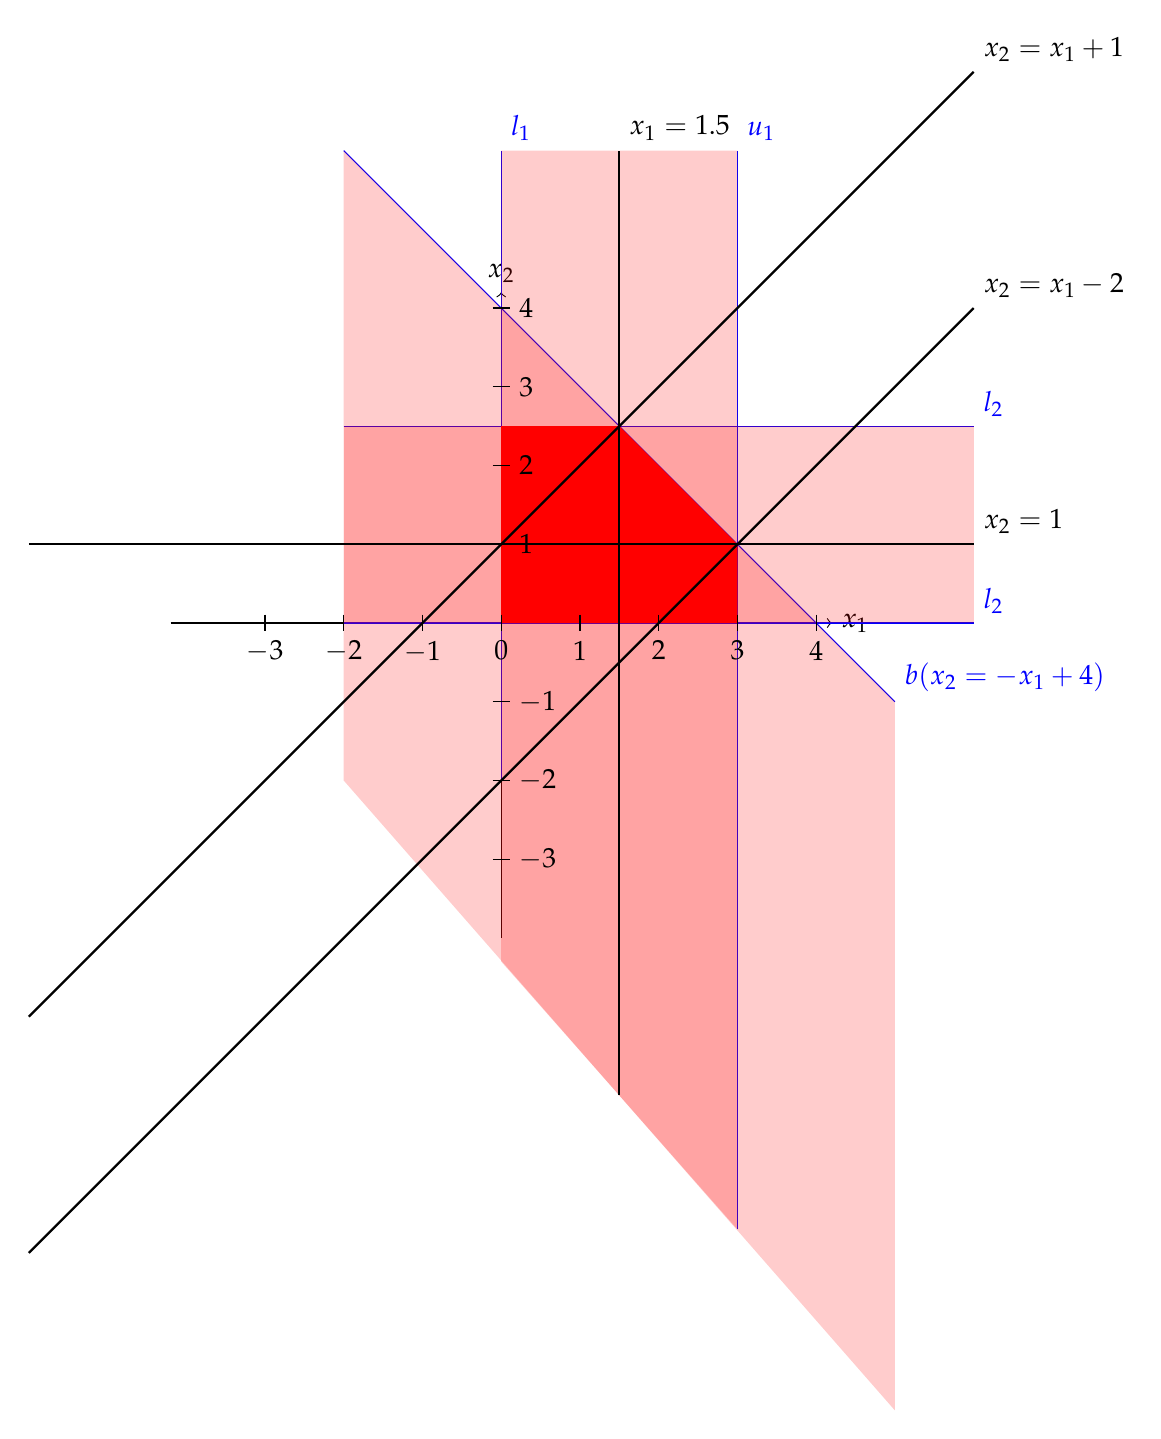
\begin{tikzpicture}
    \draw[->] (-4.2,0) -- (4.2,0) node[right] {$x_1$};
    \draw[->] (0,-4) -- (0,4.2) node[above] {$x_2$};

    
    \draw[blue] (0,0) plot[domain=-2:5] (\x,{-\x + 4}) node[anchor=south west] {$b (x_2 = -x_1 +4)$};
    \draw[blue] (0,0) plot[domain=-2:6] (0,\x) node[anchor=south west] {$l_1$};
    \draw[blue] (0,0) plot[domain=-7.7:6] (3,\x) node[anchor=south west] {$u_1$};
    \draw[blue] (0,0) plot[domain=-2:6] (\x,2.5) node[anchor=south west] {$l_2$};
    \draw[blue] (0,0) plot[domain=-2:6] (\x,0) node[anchor=south west] {$l_2$};
    
    \draw [ultra thick, draw=none, fill=red, opacity=0.2]
    (0,-4.3) -- (3,-7.7) --  (3,6) -- (0,6) -- cycle;

    \draw [ultra thick, draw=none, fill=red, opacity=0.2]
    (-2,0) -- (-2,2.5) --  (6,2.5) -- (6,0) -- cycle;

    \draw [ultra thick, draw=none, fill=red, opacity=0.2]
    (-2,6) -- (-2,-2) --  (5,-10) -- (5,-1) -- cycle;

    \draw [draw=none, fill=red]
    (0,0) -- (3,0) --  (3,1) -- (1.5,2.5) -- (0,2.5) -- cycle;
    
    
    \foreach \x in  {-3,-2,-1,0,1,2,3,4}
    \draw[shift={(\x,0)},color=black] (0pt,3pt) -- (0pt,-3pt);
    \foreach \x in {-3,-2,-1,0,1,2,3,4}
    \draw[shift={(\x,0)},color=black] (0pt,0pt) -- (0pt,-3pt) node[below] 
    {$\x$};



    \foreach \y in  {-3,-2,-1,1,2,3,4}
    \draw[shift={(0, \y)},color=black] (-3pt,0pt) -- (0pt,0pt);
    \foreach \y in {-3,-2,-1,1,2,3,4}
    \draw[shift={(0, \y)},color=black] (-3pt,0pt) -- (3pt,0pt) node[right] 
    {$\y$};

    \draw[thick, color=black] (0,0) plot[domain=-6:6] (1.5, \x) node[anchor=south west] {$x_1=1.5$};
    \draw[thick, color=black] (0,0) plot[domain=-6:6] (\x, 1) node[anchor=south west] {$x_2=1$};
    \draw[thick, color=black] (0,0) plot[domain=-6:6] (\x, \x + 1) node[anchor=south west] {$x_2 = x_1 + 1$};
    \draw[thick, color=black] (0,0) plot[domain=-6:6] (\x, \x - 2) node[anchor=south west] {$x_2 = x_1 - 2$};


    % \foreach \x in  {-3,-2,-1,1,2,3,4}
    % \draw[shift={(0,\x)},color=black] (3pt,0pt) -- (-3pt,0pt);
    % \foreach \x in {-3,-2,-1,1,2,3,4}
    % \draw[shift={(0,\x)},color=black] (0pt,0pt) -- (-3pt,0pt) node[below] 
    % {$\x$};

    \end{tikzpicture}
\subsection{Closed Form}
    Looking at chart above, it's easy so see that all points with $x_2 < 1$ or $x_1 < 1.5$ or $x_2 x_1 \leq 4$ we can 
    use box-constraints. For points between $x_2 = x_1 + 1$ and $x_2 = x_1 - 2$ and above $x_2 = -x_1 +4$ 
    we can use line projection. In every other case the projection function should return
    point $(1.5,2.5)$ or $(3,1)$ (Simple observation that those points are the nearest
    to the projection on the line, which makes them the best choice).\\


    \[ \pi_x(p) =  \begin{cases} 
        a+ \frac{(p-a)^T(b-a)}{||b-a||^2_2}(b-a)& (x_2+x_1 \gt 4) \land (x_2 - x_1 < 1) \land (x_2 - x_1 > -2)  \\
        (1.5,2.5) & x_1 > 1.5 \land (x_2 - x_1 \geq 1) \\
        (3,1) & x_2 > 1 \land (x_2 - x_1 \leq -2) \\
        min(max(l_i, p_i), u_i) & else 
     \end{cases}
    \]
    where $a$ and $b$ are lay on the $x_2 = -x_1 +4$,
\subsection{Gradient Descent}
\begin{equation}
    \nabla f(x_1,x_2) = [2x_1 - 4, 4x_2 -14]
\end{equation}
\begin{equation}
    \begin{gathered}
        \nabla f(x_0) = (1,-10) \\
        p_1 = (2.5,1) - 0.05(1,-10) = (2.45, 0.5) = x_1 \\
        p_2 = (2.45, 0.5) - 0.05(0.9, -12) = (2.405, -0.1) \\
        x_2 = \pi_x(p_2) = min(max(l_i, p_i), u_i) = (2.405, 0)
    \end{gathered}
\end{equation}
\section{Problem 3}
\subsection{Similarities}
\begin{itemize}
    \item Linear classifiers (can also be used for non-linear classification)
    \item Binary classifiers
\end{itemize}
\subsection{Differences}
\begin{itemize}
    \item SVM looks for the best possible separation. Where best is understood as
    the one that represents the largest separation between two classes. While perceptron
    looks for any separation.
    \item SVM separation is based only on few points that are are the closest to the separation line.
    Adding new points the set does not change the classification line (unless new points are "closer").
    Perceptron takes all points into the account.
\end{itemize}
\section{Problem 4}
SVN has a optimization form of minimizing:
\begin{equation}
    f_0(w,b)=\frac{1}{2} w^Tw
\end{equation}
Subject to:
\begin{equation}
    f_i(w,b) = y_i(w^Tx_i +b) - 1 \geq 0
\end{equation}
To show that duality gap is $0$ we can use weak Slater's condition which says
that strong duality holds when $f_0$ is convex and $f_i$ are affine.\\
First is satisfy as quadratic function is convex. Second is satisfy as $f_i$ are affine functions
w.r.t $w$ and $b$.
\section{Problem 5}
\subsection{Matrix $Q$}
Elementwise $g(\alpha) = \sum_i^N\alpha_i - \frac{1}{2} \sum_i^N\sum_j^N\alpha_i\alpha_jy_iy_jx_i^Tx_j$
Comparing this with vector from it's clear that $Q$ must contains $y$ and $x$ terms.
\\\\
Now we define matrix $X$ as a matrix of data points with $NxK$ shape, where $K$ is a 
number of data dimensions and $i-th$ row contains $i-th$ data point.\\
We also define matrix $Y$ with $KxN$ shape where each row is the same $y$ vector of data point class,
so that $i,j$ element of $Y$ contains class of $j-th$ data point.
\\\\
Now following is true:
\begin{equation}
    (Y^T \odot X)(Y^T \odot X)^T = \sum_i^N\sum_j^Ny_iy_jx_i^Tx_j
\end{equation}
Using above and also incorporating $-$ sign from elementwise equation we can deduce
that matrix $Q$ can by computed by following operation:
\begin{equation}
    Q = - (Y^T \odot X)(Y^T \odot X)^T
\end{equation}
\subsection{Negative semi-definiteness proof}
Matrix is negative semi-definite iff $z^TQz \leq 0$. Using matrix Q form from above
we cen rewrite this inequality as follows:
\begin{equation}
    - z^T(Y^T \odot X)(Y^T \odot X)^Tz \leq 0 
\end{equation}
Because we multiply quadratic terms in vector notation with $-$ sign at the beginning 
above is always true, thus $Q$ is negative semi-definite.
\subsection{Negative semi-definiteness consequences}
In SVN dual optimization we try to maximize $g(\alpha)$. Maximization is much
more efficient when function is concave (i.e. Have only one (global) maximum). 
Thanks to negative semi-definiteness we know that $g(\alpha)$ is concave and 
maximization problem can be solved in polynomial time (in other case the problem is NP-hard).
\end{document}
